\documentclass[journal,12pt,onecolumn]{IEEEtran}
\usepackage{cite}
 \usepackage{caption}
\usepackage{graphicx}
\usepackage{amsmath,amssymb,amsfonts,amsthm}
\usepackage{algorithmic}
\usepackage{graphicx}
\usepackage{textcomp}
\usepackage{xcolor}
\usepackage{txfonts}
\usepackage{listings}
\usepackage{enumitem}
\usepackage{mathtools}
\usepackage{gensymb}
\usepackage{comment}
\usepackage[breaklinks=true]{hyperref}
\usepackage{tkz-euclide} 
\usepackage{listings}
\usepackage{gvv}
%\def\inputGnumericTable{}                                 
\usepackage[latin1]{inputenc} 
\usetikzlibrary{arrows.meta, positioning}
\usepackage{xparse}
\usepackage{color}                                            
\usepackage{array}                                            
\usepackage{longtable}                                       
\usepackage{calc}                                             
\usepackage{multirow}
\usepackage{multicol}
\usepackage{hhline}                                           
\usepackage{ifthen}                                           
\usepackage{lscape}
\usepackage{tabularx}
\usepackage{array}
\usepackage{float}

\usepackage{float}
%\newcommand{\define}{\stackrel{\triangle}{=}}
\theoremstyle{remark}
\usepackage{circuitikz}
\captionsetup{justification=centering}
\usepackage{tikz}

\title{Matrices in Geometry 9.4.48}
\author{EE25BTECH11035 - Kushal B N}
\begin{document}
\vspace{3cm}
\maketitle
{\let\newpage\relax\maketitle}
\textbf{Question: }
Find two consecutive odd positive integers sum of whose squares is 290.

\textbf{Solution: }\\
Let the two consecutive odd positive integers be $n$ and $(n+2)$, so that we get,
\begin{equation}
    n^2 + (n+2)^2 = 290
\end{equation}

\begin{equation}
    \implies 2n^2 + 2n - 143 = 0
\end{equation}
Representing this equation as a conic section
\begin{equation}
    \vec{x}^{\top}\vec{V}\vec{x} + 2\vec{u}^{\top}\vec{x} + f = 0, \vec{V} = \myvec{1&0\\0&0}, \vec{u} = \myvec{1\\-1/2}, f = -143
\end{equation}
We need to find intersection points with $y = 0$, that is, the X-axis.
\begin{equation}
    \vec{x} = \vec{h} + k\vec{m}, \vec{h} = \myvec{0\\0}, \vec{m} = \myvec{1\\0}
\end{equation}
Substituting $\vec{x} = k\vec{m}$

\begin{equation}
    k^2\vec{m}^{\top}\vec{V}\vec{m} + 2k\vec{u}^{\top}\vec{m} + f = 0
\end{equation}

\begin{equation}
    \implies k = \frac{1}{2}\sbrak{-2\vec{u}^{\top}\vec{m} \pm \sqrt{4(\vec{u}^{\top}\vec{m})^2 - 4f\vec{m}^{\top}\vec{V}\vec{m}}}
\end{equation}

\begin{equation}
    \implies k = -\vec{u}^{\top}\vec{m} \pm \sqrt{(\vec{u}^{\top}m)^2 - f\vec{m}^{\top}\vec{V}\vec{m}}
\end{equation}

\begin{equation}
    \vec{u}^{\top}\vec{m} = \myvec{1 & -1/2}\myvec{1\\0} = 1
\end{equation}

\begin{equation}
    \vec{m}^{\top}\vec{V}\vec{m} = \myvec{1&0}\myvec{1&0\\0&0}\myvec{1\\0} = 1
\end{equation}

\begin{equation}
    k = -1 \pm \sqrt{(1)^2 - (-143)(1)}
\end{equation}

\begin{equation}
    k = -1 \pm \sqrt{144}
\end{equation}

\begin{equation}
    \implies k = -1 \pm 12 \implies \fbox{$k = 11 \text{ OR } k = -13$}
\end{equation}

Substituing $k$ into $\vec{x}$, we get
\begin{equation}
    \vec{x} = \myvec{11\\0} \text{ OR } \vec{x} = \myvec{-13\\0}
\end{equation}
This implies that the roots of the equation are 11 and -13.
So, we have
\begin{equation}
    \implies \fbox{$n = 11$}
\end{equation}

\textbf{Final Answer: }\\
$\therefore$ The two consecutive odd positive integers whose sum of squares is 290 are 13 and 11.

\begin{figure}[H]
    \centering
    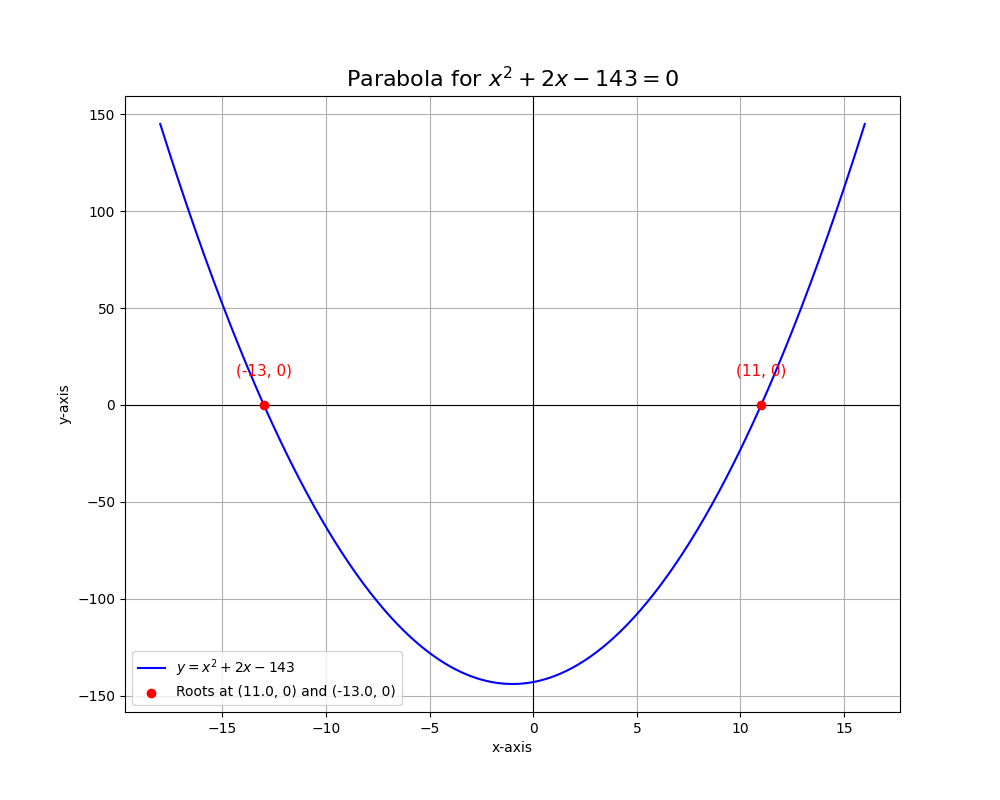
\includegraphics[width=0.80\columnwidth]{figs/1.png}
    \caption{Plot for 9.4.48}
\end{figure}
\end{document}
